\clearpage
\chapter*{Evidencia GA1-220501092-AA5-EV01: Herramienta para Gestión de Requisitos}
\phantomsection
\addcontentsline{toc}{chapter}{Evidencia GA1-220501092-AA5-EV01: Herramienta para Gestión de Requisitos}
\setcounter{section}{0}

\section{Introducción y Selección de la Herramienta}
Para la gestión de los requisitos del proyecto ``Gemelo Digital de Mantenimiento'', se ha seleccionado la herramienta \textbf{Notion} como plataforma central. La elección se basa en su capacidad para ir más allá de una simple lista de tareas, permitiendo la creación de un ecosistema de bases de datos relacionales que integran la documentación, la planificación y la trazabilidad en un solo lugar.

\section{Configuración de la Herramienta: El Ecosistema Notion}
Se ha configurado un espacio de trabajo específico para el proyecto que articula la gestión de requisitos a través de dos bases de datos principales, como se evidencia en la siguiente captura:

\begin{figure}[H]
    \centering
    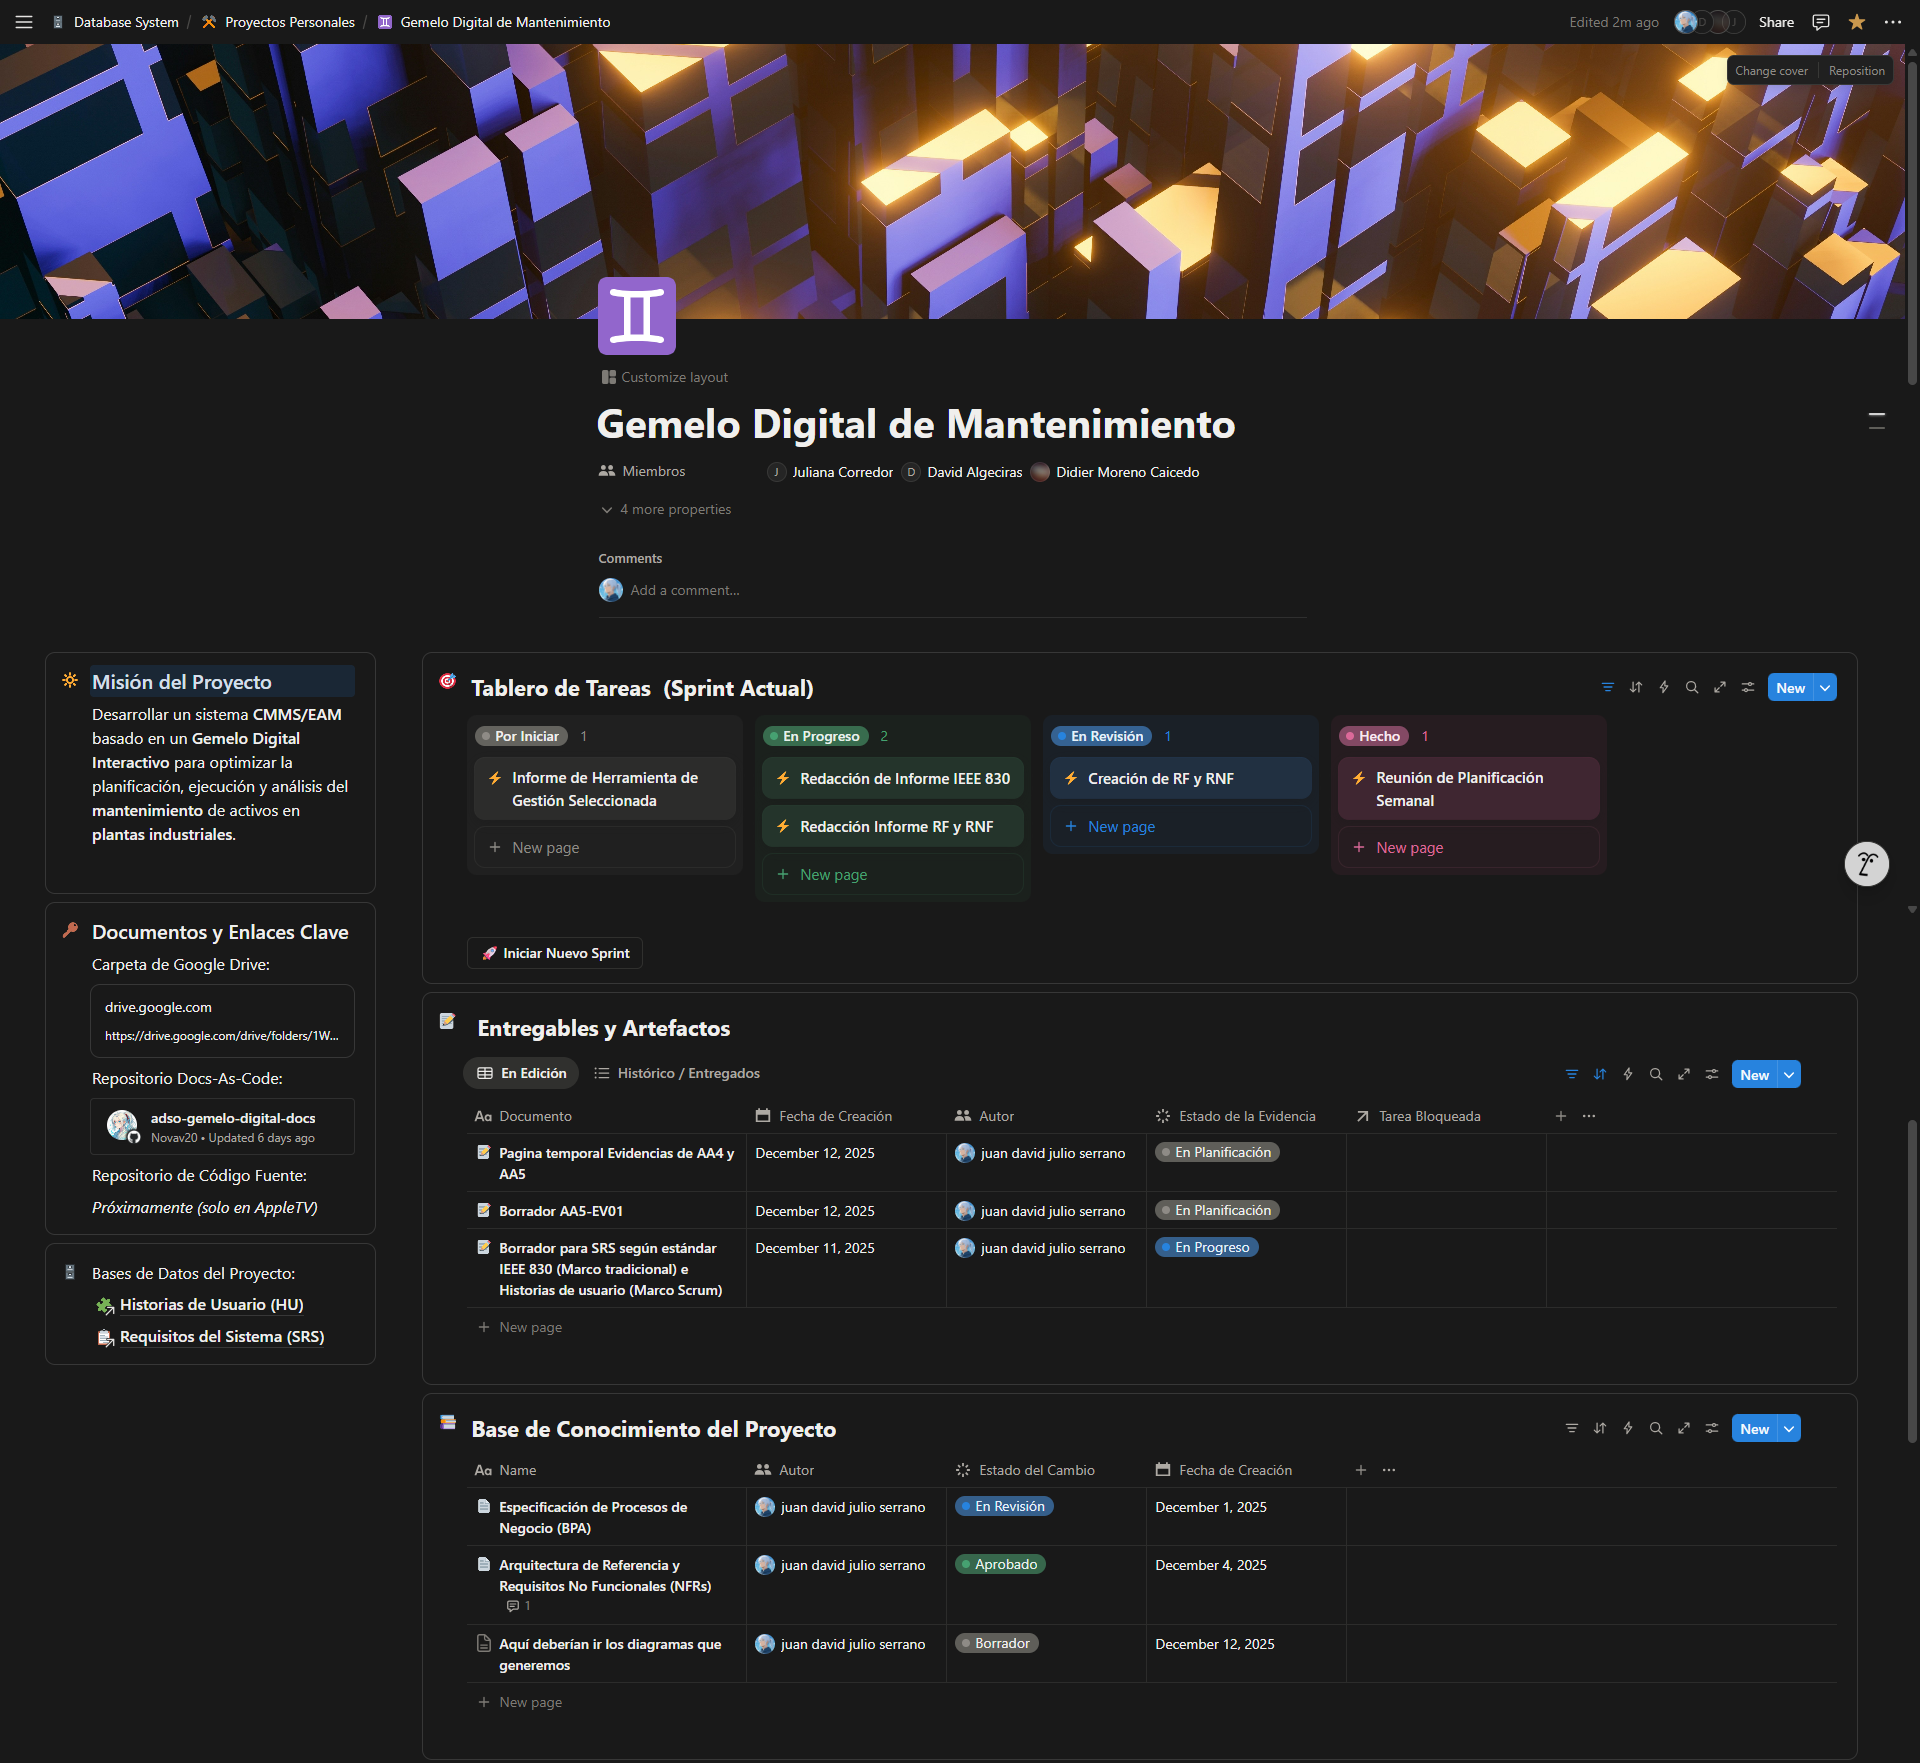
\includegraphics[width=\textwidth]{assets/notion_workspace.png}
    \caption{Espacio de trabajo en Notion}
\end{figure}

\subsection{Arquitectura de Bases de Datos}
La arquitectura se compone de:
\begin{itemize}
    \item \textbf{Historias de Usuario (HU):} Funciona como el \textit{Product Backlog}, donde cada entrada es una unidad de valor para el negocio.
    \item \textbf{Requisitos del Sistema (SRS):} Funciona como la especificación técnica, donde cada entrada es un requisito funcional (RF) o no funcional (RNF) derivado de una historia.
\end{itemize}

\subsection{Gestión de Historias de Usuario (Backlog)}
La base de datos de Historias de Usuario está configurada con propiedades para gestionar el ciclo de vida de cada funcionalidad, incluyendo ID automático, Epic (módulo), Rol y Estado.

\begin{figure}[H]
    \centering
    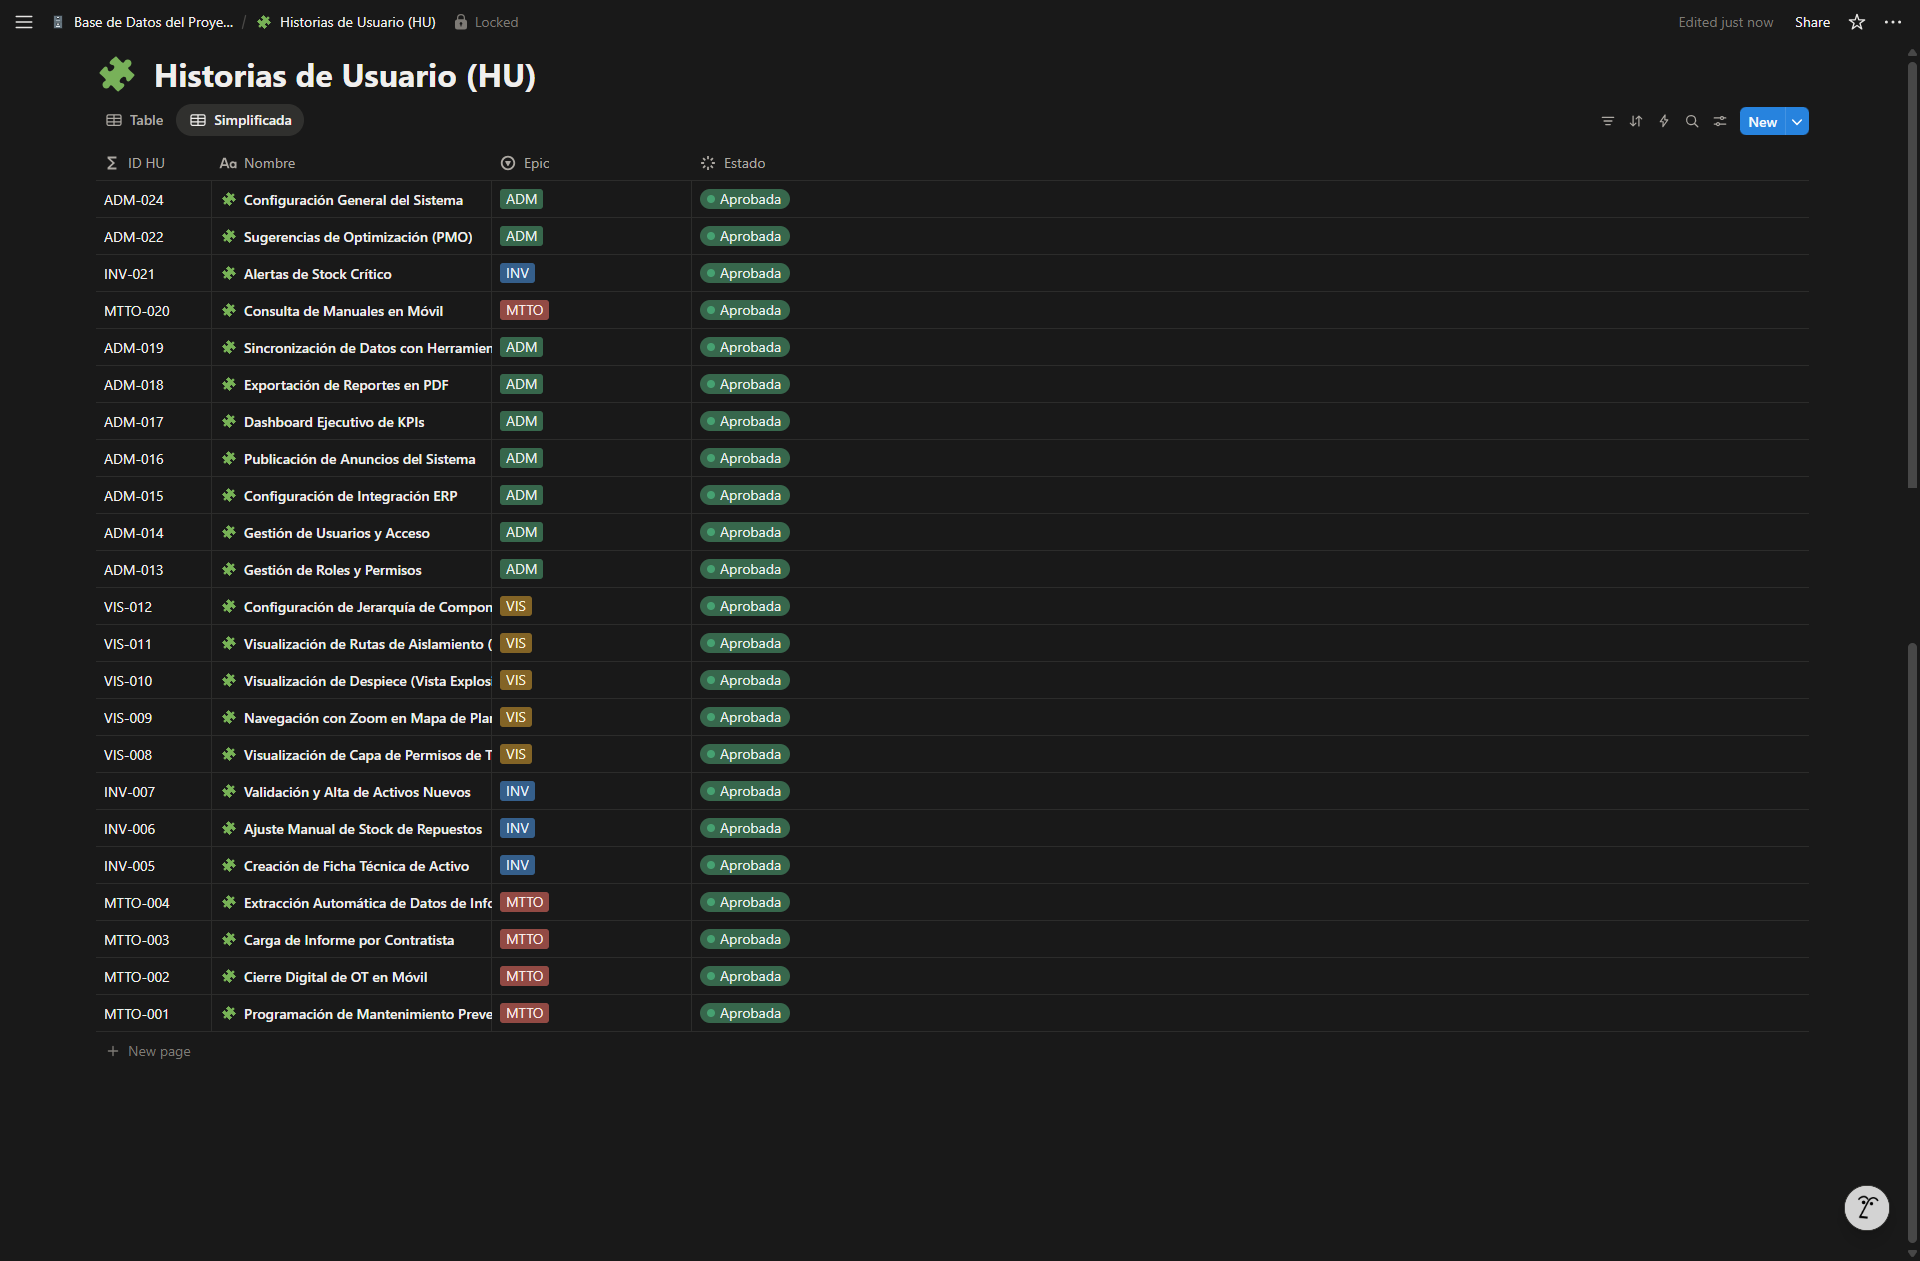
\includegraphics[width=\textwidth]{assets/notion_backlog.png}
    \caption{Gestión de Historias de Usuario}
\end{figure}

\subsection{Gestión de Requisitos (Matriz de Trazabilidad)}
La base de datos de Requisitos del Sistema permite una especificación técnica detallada y, crucialmente, la \textbf{trazabilidad}. Gracias a una propiedad de \textit{Relación}, cada requisito está vinculado a su ``Historia de Origen'', permitiendo saber siempre \textit{por qué} se está construyendo una determinada función.

\begin{figure}[H]
    \centering
    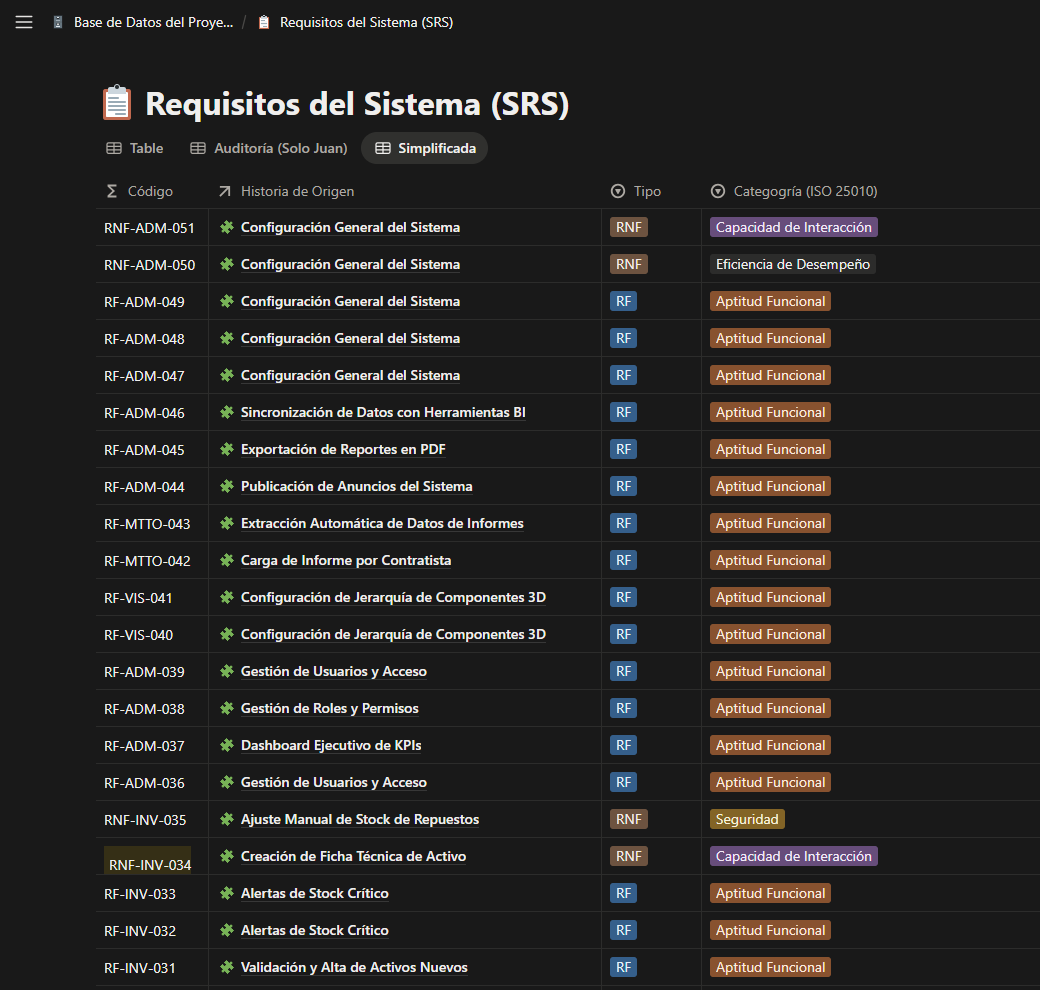
\includegraphics[width=\textwidth]{assets/notion_traceability.png}
    \caption{Matriz de Trazabilidad en Notion}
\end{figure}

\section{Justificación de la Elección}
Se eligió Notion sobre alternativas como Trello o Jira por tres razones estratégicas:
\begin{enumerate}
    \item \textbf{Integración Nativa:} Notion permite tener el ``qué'' (el requisito) y el ``cómo'' (el apunte de investigación) en el mismo lugar, eliminando la fricción de cambiar de aplicación.
    \item \textbf{Flexibilidad:} Permite crear vistas personalizadas para cada miembro del equipo, filtrando solo la información relevante para su rol.
    \item \textbf{Trazabilidad Avanzada:} La capacidad de crear relaciones bidireccionales entre Historias, Requisitos, Tareas y Documentos crea una ``matriz de trazabilidad'' viva que es imposible de lograr en herramientas más simples.
\end{enumerate}

\section{Conclusiones}
Notion ha demostrado ser una herramienta robusta y escalable para la gestión de requisitos en la fase de análisis. Su enfoque de bases de datos relacionales, en lugar de tarjetas aisladas, lo convierte en la elección ideal para un proyecto complejo que requiere un alto grado de documentación y trazabilidad.

Si bien la trazabilidad entre Historias y Requisitos está establecida, se identifican oportunidades de mejora continua, como la integración de los Criterios de Aceptación en bases de datos relacionales para facilitar las futuras fases de prueba y validación.
